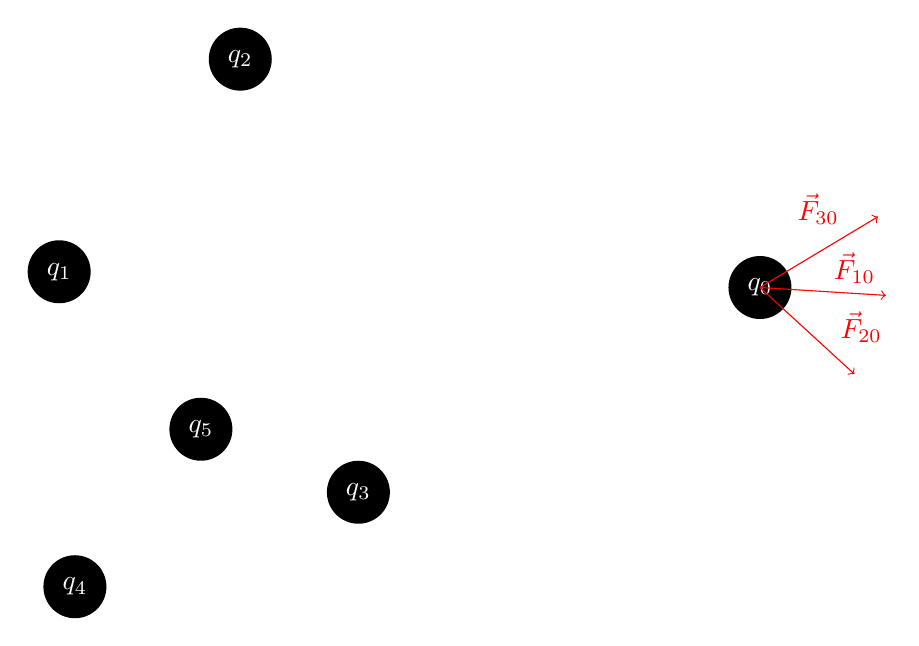
\begin{tikzpicture}
\fill  (-4.7,4.7) circle (0.4) node[white] {$q_1$};
\fill  (-2.4,7.4) circle (0.4) node[white] {$q_2$};
\fill  (-2.9,2.7) circle (0.4) node[white] {$q_5$};
\fill  (-4.5,0.7) circle (0.4) node[white] {$q_4$};
\fill  (-0.9,1.9) circle (0.4) node[white] {$q_3$};
\fill  (4.2,4.5) circle (0.4) node [white] (v1) {$q_0$};
\draw [red,->] (v1.center) -- (5.7,5.4) node [near end,above left] {$\vec{F}_{30}$};
\draw [red,->] (v1.center) -- (5.8,4.4) node [near end,above] {$\vec{F}_{10}$};
\draw [red,->] (v1.center) -- (5.4,3.4) node [near end,above right] {$\vec{F}_{20}$};
\end{tikzpicture}